\section{Analogic Quantum Computing}

\begin{frame}{Even more maths...}
The maths behin Analogic Quantum Computing (AQC) reside in the theory of complexity\newline

In a nutshell:
\begin{itemize}
    \item some "difficult" problems can be mapped as a quantum physics experiment
    \item when solving a difficult problem in a computation, we first translate it to turn it into
    one of the problems that the AQC can solve
    \item we run sevceral shots of the experiment on AQC to get a result
    \item we translate the result back into a solution of the initial problem
\end{itemize} 


Parmi les implémentations analogiques, on trouve dans le paysage actuel~:
Within the available AQC devices, and the addressable "difficult" problems, we find
\begin{itemize}
    \item supraconductionf loops in D-Wave hardware, addressing the QUBO problem
    \item cold atoms in Pasqal Hardware, addressing the MIS problem
    \item Photonics in Quandela hardware, able to compute the permaent of a matrix
\end{itemize}
\end{frame}

\begin{frame}{P and NP}
In the complexity theory, several classes of problems's complexity exiist
\begin{itemize}
    \item \textbf{P class} problems can be solved by HPC systems, they require a time to solution  varying exponentially
    with the size of the proble
    \item \textbf{NP class} problems are \textit{non-deterministic polynomial} problems, the time to solution is much 
    larger than polynomial, but checking that a candidate for a solution is an actual solution can be checked in a time
    which polynomially depends on the size of the problem. 
\end{itemize}


\textbf{BEWARE}: NP \textbf{does not mean} non-polynomial (it's quite a bad acronyl).
\end{frame}

\begin{frame}{P and NP: examples}
 P problems are addressable by regular HPC 
 \begin{itemize}
     \item computing the gcd and lcm of two very large numbers (Euclide's algorithm)
     \item inverting a matrix (Gauss's algorithm)
     \item identifying is a number is prime or not (AKS algorithm)
 \end{itemize}
NP problem: factorization of the product of two large prime numbers
 \begin{itemize}
     \item I gave you $62062883$, it's a product of two prime numbers... which ones?
     \item It's complicated... the time to solution does not vary polynomially with the number of digits
 \end{itemize}
 I make the asumption that $62062883= 7877 \times 7879$
 \begin{itemize}
     \item it's a potential solution, let's check it!
     \item checking it is fast... we do a mulitplication (which is clearly a polynomial problem)
 \end{itemize}
Factorization is a typical NP problem
\end{frame}

\begin{frame}{The Complexity Zoo}
\centering
    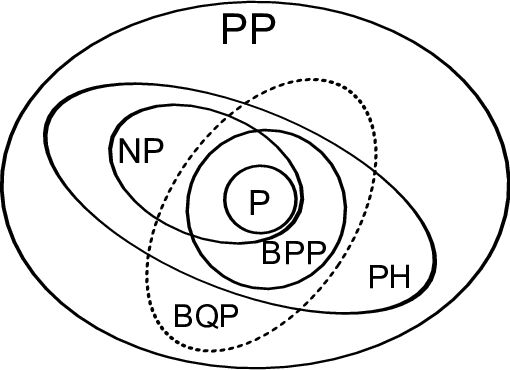
\includegraphics[width=9cm]{
        images/A-diagram-for-the-relations-between-complexity-classes-P-NP-PH-BPP-PP-and-BQP-Note.png}
\end{frame}

 \begin{frame}{NP Complete problems - Cook's theorem}
By definition, a \textbf{NP-hard} problem is so that any NP problem can be translated into this problem. By solving it,
you solve any NP problem. \newline \newline

\textbf{Definition:~} A problem which is both NP and NP-hard is \textbf{NP-Complete}. \newline \newline

The Cook's Theorem (demonstrated in 19771) styates that NPC problems exis, and that converting a NP problem into a NPC one
in a probem whose complexity is of class P (addressable by HPC). \newline \newline

Many NP-Complete probems have been identified (QUBO, Travelling Salesperson (TSP), SAT, MIS, ...), in 1972 the
Karp's list shows 21 of them
\end{frame}

\begin{frame}{Karp's list 1/2}
In 1972, right after the demonstration of the Cook's theorem in 1972, Karp lists 21 NP-Complete problems.
\begin{itemize}
    \item SATISFIABILITY : The SAT problem, the basement of Cook's demonstration
    \item CLIQUE : detecting a "clique" (similar to a social network community) in a graph
    \item SET PACKING 
    \item VERTEX COVER 
    \item SET COVERING
    \item FEEDBACK ARC SET 
    \item FEEDBACK NODE SET 
    \item DIRECTED HAMILTONIAN CIRCUIT 
    \item UNDIRECTED HAMILTONIAN CIRCUIT
    \item INTEGER PROGRAMMING 
    \item 3-SAT 
     \item CHROMATIC NUMBER : finding the "chromatic number" for a graph
\end{itemize}
\end{frame}

\begin{frame}{Karp's list 2/2}
\begin{itemize}
    \item CLIQUE COVER 
    \item EXACT COVER
    \item MATCHING à 3 dimensions 
    \item STEINER TREE 
    \item HITTING SET 
    \item KNAPSACK 
    \item JOB SEQUENCING 
    \item PARTITION 
    \item MAX-CUT 
    \item QUBO
    \item TSP: Traveling Sales Person
\end{itemize}    
\end{frame}

\begin{frame}{QUBO and Simulated Annealing}
\textbf{Q}uadratic \textbf{U}nconstrained \textbf{B}inary \textbf{O}ptimisation focuses on finding optimum of a 
quadratic function (expressed as a real matrix) whose input is a binary vector.
\newline

QUBO is NPC, but it can be approximated since 1984 by textit{Simulated Annealing} method. The algorithm's name 
derive from metallurgy. 
\newline

Simulated Annealing derives from Metropolis-Hastings algorithm, which focuses on thermodynamics. Many implementation
exists (including Mathematica). Its existence since a long time explains why so many "convert to QUBO" methods exist
when it comes to solving NPC problems
\newline

QUBO is natively implented by D-Wave hardware which is capable of providing exact solution of QUBO. 
\end{frame}

\begin{frame}{Le problème Max-Cut 1/2}
Knowing a graph $G=(V ; E)$, made of vertices connected by edges, we want to do the \textit{Maxium Cut}: separate the 
set of vertices $V$ in two complementary parts $V_1$ and $V_2$, so that the set of edges connecting vertices from
$V_1$ and $V_2$ is the largest one. 
\newline

MaxCut can be enhanced by adding \textit{weights} on each edge. It then possible to define a global weight associated with 
a cut. MaxCut will then try to find the cut with the highest global weight.
\centering
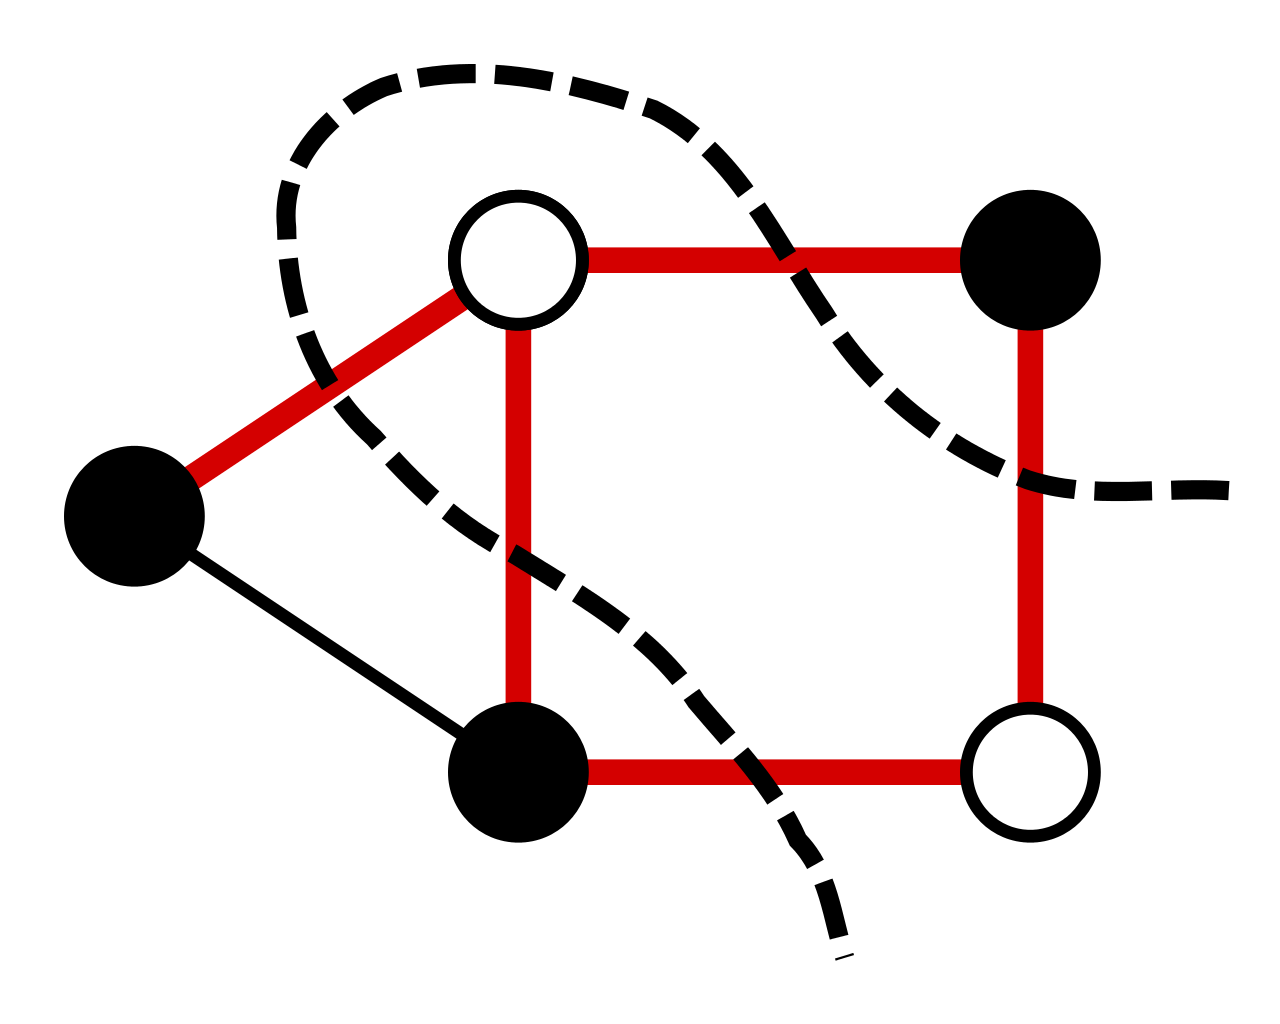
\includegraphics[width=7cm]{images/Max-cut.svg.png}
\end{frame}

\begin{frame}{Le problème Max-Cut 2/2}
\textbf{Remark:} We can define Mincut in a completely similar way.

MaxCut, and the discovery of a maximum cut in a graph is associated with:
\begin{itemize}
    \item decision making problem~: knowing a grap $G$, is there is an integer $k$ such as a cut whose weight is at least $k$
    \item optimisation problem : knowing a graph $G$, find the cut with the highest cut
\end{itemize}

MaxCut has complexity P if the involved graph is \textit{planar} (its dimension is 2); \newline


As graph become more complex, MaxCut is NP-Complete (both NP and NP-hard)
\end{frame}

\begin{frame}{The MIS problem}
Knowing a graphe $G = (V ; E)$, what is the largest set of \textit{independent} vertices, such no edge exist between
any two different elements of this \textit{Maximum Independent Set}.

Sometimes, several different solutions exist 
Il existe souvent plusieurs solutions à ce problème.
\newline

MIS are dominants subsets. A subset of vertices $S$ of a graph is dominant is any vertex is either in $S$, or connected 
(neighbour) to a element in $S$. MIS arte the largets dominant subsets.

\centering
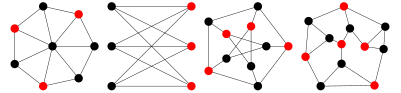
\includegraphics[scale=0.8]{images/MaximumIndependentSet_1000.png}
\end{frame}

\begin{frame}{The MVC problem}
MVC stands for \textit{Maximum Vertex Cover}, it is dual with the MIS problem. 

A cover of vertices is a subset of vertices, it is defined as \textit{transversal} in $G$ if any edge in $E$ connects
to at least one element in the cover. MVC aims to find the smallest transveral cover. 
\newline

Analogy: edges are corridors, verices are "crossroads", where should I installed cameras in order to watch all the 
corridors?

\centering
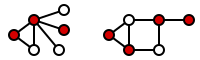
\includegraphics[scale=1.0]{images/Vertex-cover.svg.png}
\end{frame}

\begin{frame}{The SAT problem}
SAT is involved in Cook's theorem's demonstration. Knowing boolean (true or false) variable, we can design a 
\textit{proposition}: a formula using this variables with logicial AND ($\land$) and OR ($\lor$) operator. 
\newline
SAT problem asks this : knowing a proposition, does it have solution? It's not aabout finding solution or counting solutions,
it about knowing if a solution exists. This is why it's call \textit{boolean satisfiability}.
\newline
Example:  $(p\land q)\lor \lnot p$ has result $true$ if $p$ is $false$, with any value for $q$, it can be \textbf{satisfied},
but $(p\land \lnot p)$ has no solution, it can't be satisfied. 

SAT is P with simple proposition, when the proposition's \textit{atoms} involve only two variables, it's 2-SAT. 2-SAT is P.

3-SAT is NP-Complete. Any larger SAT problem can be converted into 3-SAT by increasing the number of variables. 

\end{frame}

\begin{frame}{NP conversion: solving MacCut with QUBO 1/2}

Let's consider this graph with 4 fours and weighted edges.

\centering
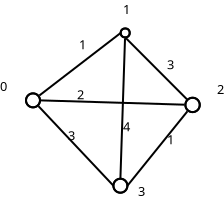
\includegraphics[scale=0.7]{images/graph4pt.png}
\end{frame}

\begin{frame}{NP conversion: solving MacCut with QUBO 2/2}
We can translate the graph into its \textit{connectivity matrix} whose coefficients  $w_{ij}$ are defined by
\begin{itemize}
    \item 0 if $i = j$ 
    \item the weight of the edge connecting  if $i \neq j$ and an efge exist
    \item 0 if no edge exist between nodes $i$ and $j$
\end{itemize}
In our exqmple, we'll build this matrix
\begin{equation*}
 W = \begin{pmatrix}
         0 & 1 & 2 & 3 \\
         1 & 0 & 3 & 4 \\
         2 & 3 & 0 & 1 \\
         3 & 4 & 1 & 0 \\
     \end{pmatrix}    
\end{equation*}
Knowing a graph cut, input binary $b$ has coefficients $b_i$: $1$ if node $i$ is in the cut, 0 otherwise.
Solving MaxCut can be reduced as solving QUBO using the quadratic function associated with the connectivity matrix.
We'll look for the maximum. 
\end{frame}

\begin{frame}{NP conversion: solving 3-SAT with MIS 1/3}
3-SAT can be solved via a MIS problem. 

Let's consider a conjonctive and normal propositiion involving $n$ variables and $m$ clauses.  

\begin{itemize}
    \item for each clause, a small 3 vertices graph is built, each vertex is a variable or the negate of a variable
    \item those small graph are linked by connected a variable in a 3 vertices graph with its negate in another
    3 vertices graph
\end{itemize}
Example: let's consider  $\lnot x_1 \lor x_2 \lor x_3$, it will be depicted by this graph


\centering
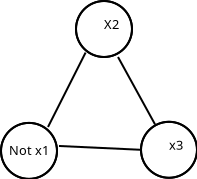
\includegraphics[scale=0.25]{images/Clause3SAT.png}
\end{frame}

\begin{frame}{NP conversion: solving 3-SAT with MIS 2/3}
We connect sub-graphes together by connected $v$ with $\lnot v$

Let's consider
suivante
\begin{equation*}
    (x_1 \lor x_2 \lor x_3) 
    \land (\lnot x_1 \lor x_2 \lor x_3 ) 
    \land (x_1 \lor \lnot x_2 \lor x_3 )
    \land (\lnot x_1 \lor x_2 \lor \lnot x_3 )
\end{equation*}
\centering
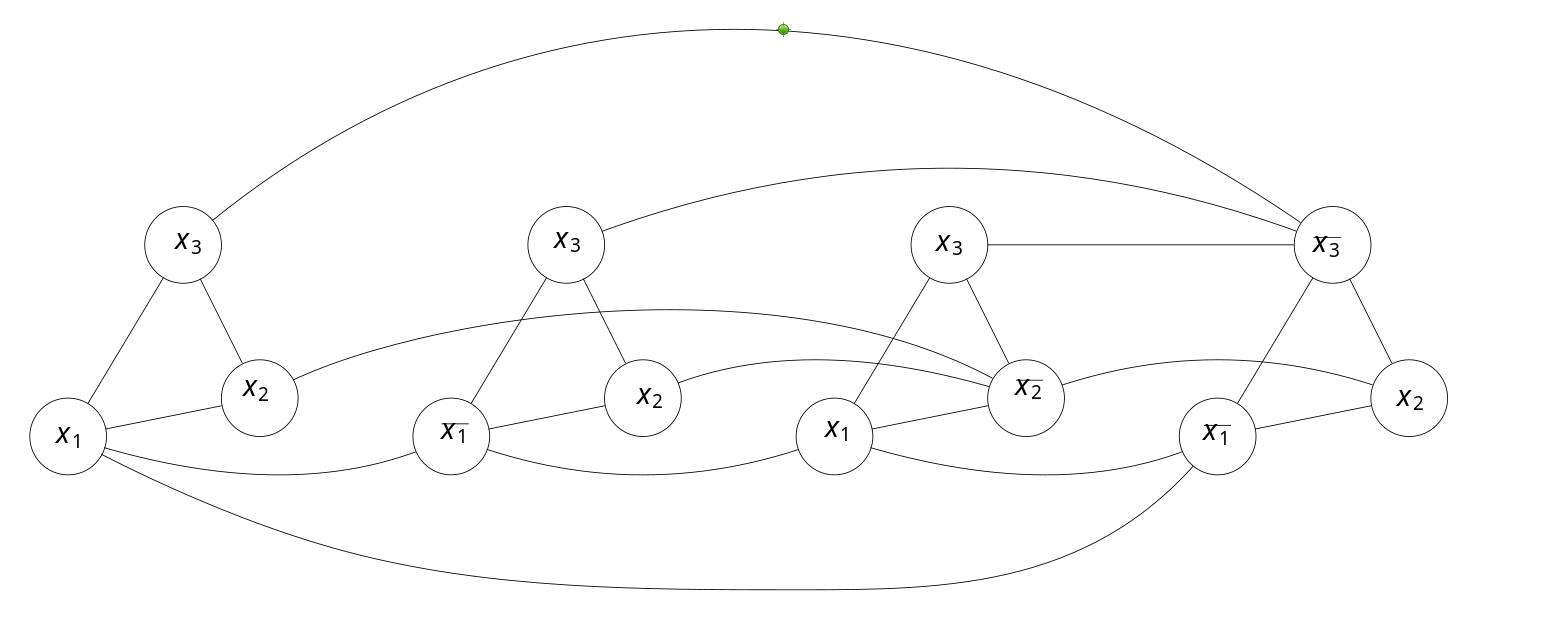
\includegraphics[scale=0.25]{images/Graphe-Clause3SAT.png}
\end{frame}

\begin{frame}{NP conversion: solving 3-SAT with MIS 3/3}
By solving MIS on the resulting graph, we can evaluate the size of this maximum set and compare it to the number of clauses
within the original proposition. If values are the same then the proposition can be satisfied. 


If the MIS size is smallest than the number of clauses, then the proposition can't be satisfied.
\end{frame}

\begin{frame}{NP problems are everywhere}
NP problem are very common in graph theory or in optimisation related problems.

They are often "simple to describe" but "hard to solve".
\begin{itemize}
    \item Traveling Sales Person (TSP) is very interesting for logistics 
    \item Clique problem is very interesting for Social Networks: cliques describe users's community
    \item Many optimisations problem, involving \textit{cost functions}, can be solved as a QUBO
    \item MaxCut is associated with decision making algorithms
\end{itemize}

If any "NP to NPC" conversion is P (Cook's theorem), designing this conversion is very difficult. Many conversion to 
QUBO exist, because QUBO could be approximated since 1984 and was an early point of interest. 
\end{frame}


\begin{frame}{Back to the MIS problem}
The Pasqal hardware can natively address the \textit{Maximum Independant Set} (MIS) problem
\begin{itemize}
    \item let's consider a graph $(G ; E)$
    \begin{itemize}
        \item $G$ is a set of points, or \textit{vertices} in a $n$ dimensions field
        \item $E$ is a set of segments connecting two vertices, or \textit{edges}
    \end{itemize}
    \item we look for the largest set(s) of vertices that are not connected (no edge exist between any two points
    in the MIS)
\end{itemize}

With pasqal hardware, a hardware constraint exist: the graph should be \textit{Unitary Disk Graphs} (UDG), associated 
with a \textit{radius} $R$
\begin{itemize}
    \item vertices whose distance is lower than $R$ are necessarily connected
    \item if two vertices are connected (an edge exists) then the distance between them is lower than $R$
\end{itemize}

This MIS problem is dual to the \textit{Minimum Vertices Cover} (MVC)
\begin{itemize}
    \item in MVC, we want to identfy the smallest set of vertices where "cameras" should be places to see all of the
    edges within a graph.
    \item we can demonstrated that MVC and MIS have no common points and their union is the whole graph.
\end{itemize}
\end{frame}    

\begin{frame}{Pasqal hardware: the physics behind the stage}
The Pasqal system  uses some Quantum Physics phenomenons, which can be mapped to MIS
\begin{itemize}
    \item monovalent (only one electron) Rubidiu atoms are emitted in a void chamber, lasers slow them down and
    place them as "optical tweezers"
    \item the lowest highest excitation level of the electron implement the states $\ket{0}$ and $\ket{1}$
    \item atoms are entangled by thee \textit{Rydberg blocade} mechanism
    \item atoms whose state is $\ket{1}$ can be jected (but we knwow where they have been placed)
    \item with a special camera, remaining atoms are seen using fluorescence 
\end{itemize}
Meanwhile
\begin{itemize}
    \item Atoms have to be within a \textit{Rydberg Radius} in order to be entangled
    \item entangled atoms are in global state $\frac{1}{\sqrt{2}}(\ket{01}+\ket{10})$
\end{itemize}
\end{frame}

\begin{frame}{The Pulser API is not user friendly}
The Pulser API is kind of "control command" related API
\begin{itemize}
    \item it locates the atoms on a grid
    \item it sets the Rydberg Radius by tweaking the correct laser frequencies
    \item it sets the shape of the laser wavelenghts (or \textit{pulses}) used to excitate the atoms  
    \item many shots and related observations are done
\end{itemize}
Pulser does not actual define a "program", it's an advanced toolkit that program the experiment environment for the 
Pasqal system
\end{frame}

\begin{frame}[fragile]
\frametitle{Code sample - Initialisation}
The init of the Pulser python framework looks like this
\newline
\begin{verbatim}
import numpy as np
from pulser import Pulse, Sequence, Register
from pulser_simulation import Simulation
from pulser.devices import MockDevice
from pulser.waveforms import RampWaveform, ConstantWaveform

import matplotlib.pyplot as plt
import qutip
\end{verbatim}
\end{frame}

\begin{frame}[fragile]
\frametitle{Code sample - Graph descriptio,}
\begin{verbatim}
# Define a dictionary where each key is the name of the qubit,
# and each value is the qubit's position (in um)

qubit_positions = {
    'q0': (0, 0),
    'q1': (3, 5.2),
    'q2': (6, 0),
    'q3': (9, -5.2)
}
\end{verbatim}

Ce dictionnaire est ensuite transformé en registre.
\\
\begin{verbatim}
# Arrangements of qubits on the machine are called a register
# Define a register in Pulser by passing the qubit dictionary
reg = Register(qubit_positions)
reg.draw()
\end{verbatim}
\end{frame}

\begin{frame}[fragile]
\frametitle{Set the Graph Radius / Rydberg Radius}
\begin{verbatim}
# Define the maximum Rabi frequency via a blockade radius
blockade_radius = 8.7
Omega_max = MockDevice.rabi_from_blockade(blockade_radius)

# Visualize the edges induced by the chosen blockade radius
reg.draw(blockade_radius=blockade_radius)
\end{verbatim}
\begin{center}
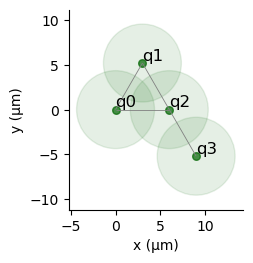
\includegraphics[scale=0.60]{images/reg3.png}
\end{center}

\end{frame}

\begin{frame}[fragile]
\frametitle{Define laser pulses}
\begin{small}
\begin{verbatim}
# A Sequence is the object that contains all
# the info about the quantum evolution
seq = Sequence(reg, MockDevice)

# Now we want to fill the channel with pulses 
# First we need to define the waveforms for the pulses
# First ramp
omega_wf_1 = RampWaveform(300, 0, Omega_max) 

#arguments are duration (ns), detuning (rad/us)
delta_wf_1 = ConstantWaveform(300, -40) 

first_pulse = Pulse(omega_wf_1, delta_wf_1, 0)
seq.add(first_pulse, 'ch')
seq.draw()
\end{verbatim}
\end{small}
\end{frame}

\begin{frame}{Shapes of the wavelengths}
The laser pulses will look like this
\begin{center}
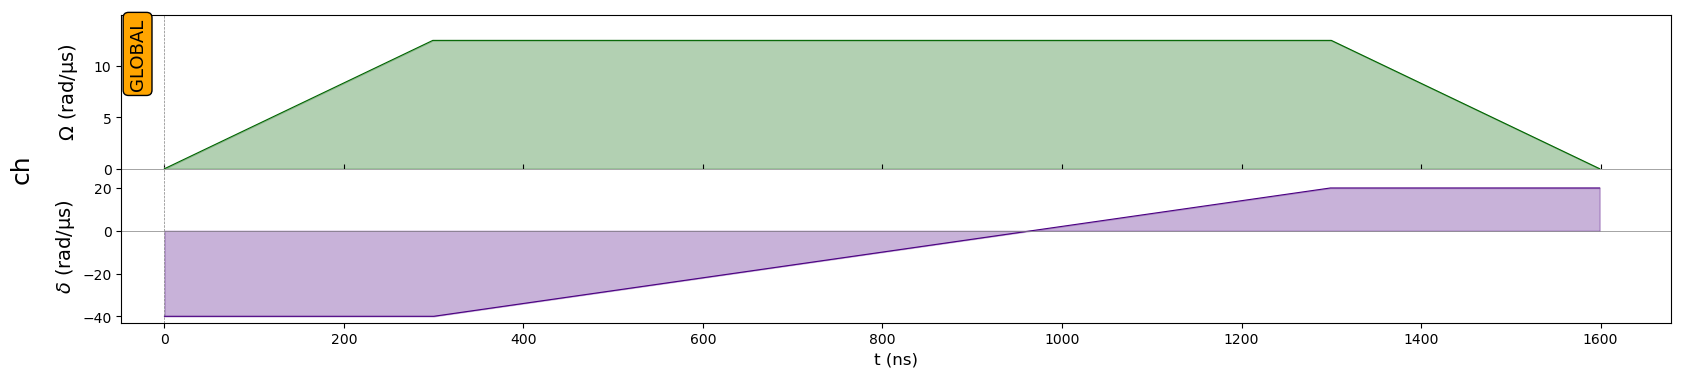
\includegraphics[scale=0.30]{images/seq1.png}
\end{center}
\end{frame}

\begin{frame}[fragile]
\frametitle{Pulser - end of code}
\begin{verbatim}
# The sequence is ready now for simulation

sim = Simulation(seq)
results = sim.run()

# The result can be sampled
samples = results.sample_final_state(10000)

# And the sampling can be visualized
plt.bar(samples.keys(), samples.values())
\end{verbatim}
\end{frame}

\begin{frame}{Results}
We finally get the final result
\begin{center}
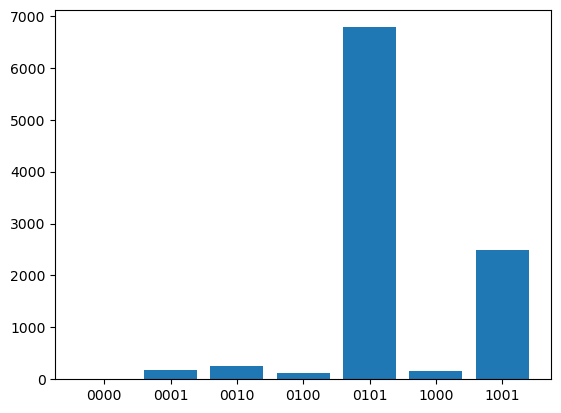
\includegraphics[scale=0.5]{images/histo1.png}
\end{center}
On voit deux solutions : $\ket{0101}$ et $\ket{1001}$. ce sont les solutions du problème MIS.
\end{frame}

\begin{frame}{AQC middle is a requirement}
AQC devices are less sensitive to noise or decoherence, when compared to gate based machines, but the interface operates
at a very low level
\begin{itemize}
    \item pieces of middleware are required to translate a user's NP problem into MIS
    \item pieces of middleware are required to translate a MIS input into a Pulser experiment
\end{itemize}
One of the challenges to future AQC systems will be related to this software integration, mixing HPC and QC since
HPC systems will do all of the "translate stuff". Many things are still to be done. 
\end{frame}

